\documentclass[UTF8]{article} % For LaTeX2e
\usepackage{CTEX}
\usepackage{caption}
\captionsetup[table]{name=Table}
\captionsetup[figure]{name=Figure}
\renewcommand{\refname}{References}
\usepackage{graphicx}
\usepackage{makecell}
\usepackage{tabularx}

\usepackage{iclr2026_conference,times}

% Optional math commands from https://github.com/goodfeli/dlbook_notation.
\input{math_commands.tex}

\usepackage{hyperref}
\usepackage{url}


\title{CriticPilot: GenPilot with Planner-Critic Mechanism}

% Authors must not appear in the submitted version. They should be hidden
% as long as the \iclrfinalcopy macro remains commented out below.
% Non-anonymous submissions will be rejected without review.

\author{
\textbf{Yan Haopeng(颜皓鹏) 24300240240} \\
\textbf{Li Zedong(李泽栋) 23307130271} \\
\textbf{Shen Zixuan(沈子轩) 24300240213} \\
Department of Computer Science \\
Fudan University
}

% The \author macro works with any number of authors. There are two commands
% used to separate the names and addresses of multiple authors: \And and \AND.
%
% Using \And between authors leaves it to \LaTeX{} to determine where to break
% the lines. Using \AND forces a linebreak at that point. So, if \LaTeX{}
% puts 3 of 4 authors names on the first line, and the last on the second
% line, try using \AND instead of \And before the third author name.

\newcommand{\fix}{\marginpar{FIX}}
\newcommand{\new}{\marginpar{NEW}}

%\iclrfinalcopy % Uncomment for camera-ready version, but NOT for submission.
\begin{document}
\iclrfinalcopy

\maketitle

\begin{abstract}

Test-time prompt optimization in text-to-image generation aims to
improve prompts through iterative refinement to make generated images
more accurately match user intent. However, existing methods like
GenPilot adopt a linear feed-forward pipeline lacking internal
verification mechanisms, facing two core bottlenecks: error overload and
history pollution. Inspired by PixelCraft\textquotesingle s
Planner-Critic architecture, this paper proposes CriticPilot, a
lightweight extension to GenPilot. CriticPilot embeds three core modules
into the original optimization process: an error aggregator, L1 local
retry, and L3 global reset, endowing the system with self-correction
capabilities. Experiments on 10 batches of complex prompts demonstrate
that CriticPilot achieves an average score improvement of 0.4118 points
(13.3485 → 13.7604), while reducing average evaluation rounds by 1.5,
validating the effectiveness and efficiency of the proposed mechanisms.

\textbf{Open Source Code}:

\url{https://github.com/zdleeeeee/PlannerCritic-GenPilot}

\end{abstract}

\section{Introduction}\label{introduction}

The field of text-to-image (T2I) generation has made significant
progress in recent years, but enabling generated images to accurately
match complex textual descriptions remains an open challenge. Test-Time
Prompt Optimization, as a lightweight solution that requires no model
fine-tuning, has garnered widespread attention by iteratively improving
prompts to enhance generation quality.

Genpilot \cite{ye2025genpilotmultiagenttesttimeprompt} is a representative work in this field,
leveraging multimodal large language models to conduct fine-grained
error analysis on generated images and generate correction suggestions
accordingly, achieving excellent results on multiple benchmarks.
However, GenPilot employs a \textbf{linear feed-forward pipeline}
lacking internal verification mechanisms. As the authors acknowledge,
VQA-based error detection is unreliable in complex scenarios. Once
early-round error analysis deviates, subsequent optimization builds upon
erroneous premises, leading to problem accumulation without the ability
to self-correct.

Specifically, GenPilot faces two core bottlenecks:

\begin{itemize}
\item
  \textbf{Error Overload}: Fine-grained error analysis may generate
  numerous redundant error descriptions (measured at over 500 for a
  single prompt segment), causing optimization objectives to diverge and
  key correction directions to be obscured.
\item
  \textbf{History Pollution}: The linear cumulative optimization
  paradigm continuously propagates error modification records generated
  during early iterations to subsequent rounds. Once early deviations
  from the correct direction occur, errors accumulate continuously,
  ultimately causing scores to stagnate at local optima.
\end{itemize}

Inspired by PixelCraft \cite{zhang2025pixelcraftmultiagenthighfidelityvisual}---which introduces a critic agent to
review reasoning trajectories and triggers backtracking when errors are
detected---this paper proposes \textbf{CriticPilot}, an extension to
GenPilot. CriticPilot embeds the Planner-Critic mechanism into the
original optimization process, endowing the system with self-correction
capabilities through error aggregation and hierarchical backtracking,
achieving an efficient closed loop for test-time prompt optimization.
Experiments demonstrate that CriticPilot achieves an average score
improvement of 0.4118 points across 10 batches of complex prompts while
reducing average evaluation rounds by 1.5.

The main contributions of this paper are as follows:

\begin{enumerate}
\def\labelenumi{\arabic{enumi}.}
\item
  Identified the two bottlenecks of error overload and history pollution
  in GenPilot\textquotesingle s linear optimization process;
\item
  Proposed CriticPilot, a lightweight self-correction framework
  incorporating an error aggregator, L1 local retry, and L3 global
  reset;
\item
  Validated the effectiveness and efficiency of the proposed mechanisms
  across multiple complex prompt batches.
\end{enumerate}

\section{Related Work}\label{related-work}

\subsection{GenPilot: Test-Time Prompt
Optimization}\label{genpilot-test-time-prompt-optimization}

GenPilot \cite{ye2025genpilotmultiagenttesttimeprompt} is a multi-agent test-time prompt
optimization system that iteratively improves prompts through two
stages: the \textbf{error analysis stage} utilizes VQA and Captioning
agents to identify semantic inconsistencies between generated images and
prompts; the \textbf{prompt optimization stage} generates multiple
candidate corrections, selects the optimal one through scoring and
clustering, and proceeds to the next iteration.

\textbf{Limitations}: GenPilot\textquotesingle s process is strictly
linear with no process-level verification mechanisms. As stated in the
paper, "VQA-based error detection is unreliable in complex scenarios."
If deviations occur during the error analysis stage, subsequent
optimization builds upon erroneous premises, and the system cannot
detect or recover from them.

\subsection{PixelCraft: Planner-Critic
Architecture}\label{pixelcraft-planner-critic-architecture}

PixelCraft \cite{zhang2025pixelcraftmultiagenthighfidelityvisual} 
is a multi-agent visual reasoning system
whose core innovation lies in its \textbf{Planner-Critic architecture}:
a critic agent (Critic) is responsible for reviewing the
planner\textquotesingle s (Planner) reasoning trajectory, detecting
inefficiencies or errors in tool usage sequences, and triggering
backtracking and branch exploration when problems are discovered.
Specific mechanisms include: (1) \textbf{Posterior refinement}: the
critic reviews the entire reasoning trajectory after discussion
completion; (2) \textbf{Backtracking and branching}: through image
memory storing intermediate results, the planner can backtrack to
previous steps when encountering contradictions and explore other
reasoning paths.

This paper draws upon PixelCraft\textquotesingle s core ideas, adapting
them to the prompt optimization domain---replacing explicit Critic LLMs
with error aggregation and score stagnation detection to achieve similar
self-correction capabilities in a lightweight manner.

\section{Method}\label{method}

CriticPilot inserts three core modules into GenPilot\textquotesingle s
standard optimization loop, with the overall architecture shown in
Figure 1.

\begin{figure}[htbp]
    \centering
    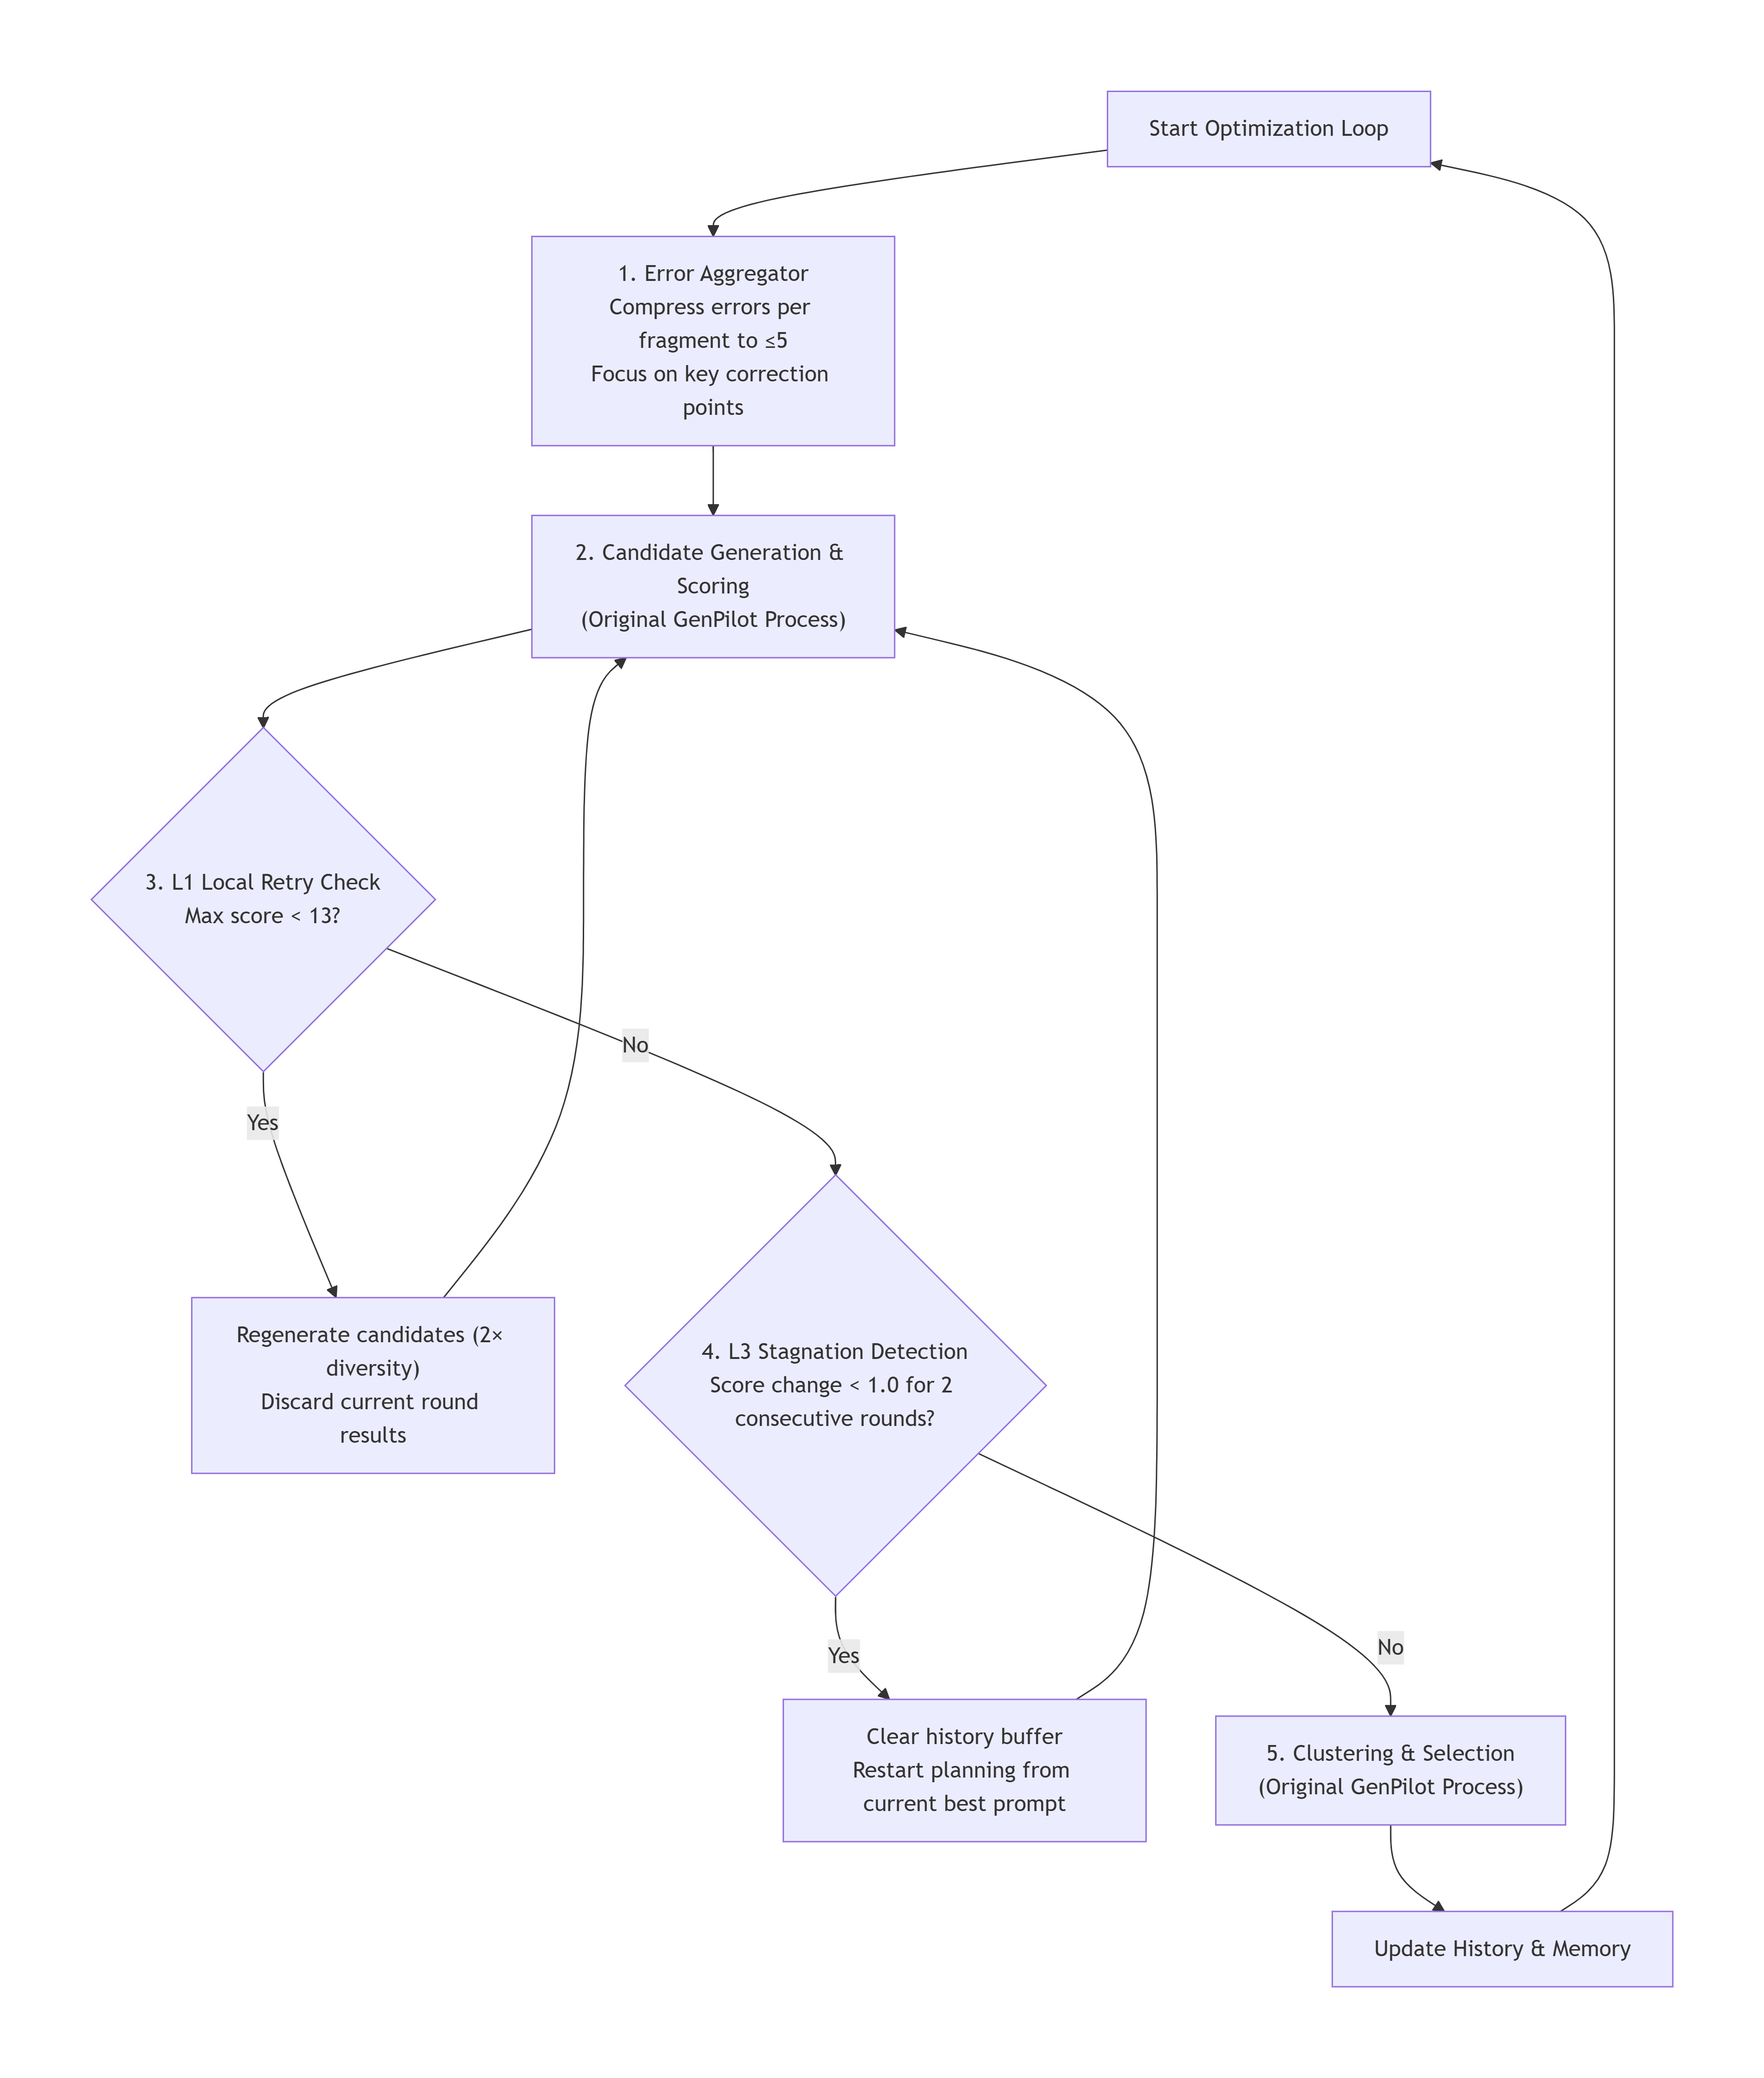
\includegraphics[width=0.8\linewidth]{../overall/CriticPilotArchitecture.png}
    \caption{CriticPilot Architecture Overview}
    \label{fig:bottle_body}
\end{figure}

\subsection{Error Aggregator}\label{error-aggregator}

\textbf{Problem}: Fine-grained error analysis may generate numerous
redundant errors (measured at over 500 for a single segment), causing
optimization objectives to diverge.

\textbf{Method}: Before each round of optimization, perform semantic
clustering on all error feedback related to the current prompt,
deduplicate by dimensions such as entity and attributes, and constrain
the number of errors associated with each prompt segment to no more than
5.

\textbf{Effect}: Compresses redundant errors by an order of magnitude,
focusing on key correction points and fundamentally avoiding
optimization signal overload.

\subsection{L1 Local Retry}\label{l1-local-retry}

\textbf{Problem}: Candidate prompts generated in a single round may have
overall low quality (e.g., due to sampling randomness).

\textbf{Detection Condition}: The highest score among all candidate
prompts in the current round is less than 13 (out of 15 points).

\textbf{Action}: Discard the current round\textquotesingle s results and
regenerate candidates with higher diversity in the same optimization
context (candidate count doubled).

\textbf{Design Rationale}: Drawing from PixelCraft\textquotesingle s
"branching" concept, conducting branch exploration at the micro-level to
rescue low-quality rounds caused by sampling randomness at low cost.

\subsection{L3 Global Reset}\label{l3-global-reset}

\textbf{Problem}: Historical modification records (history buffer) may
be contaminated by erroneous information, causing optimization to become
trapped in local optima.

\textbf{Detection Condition}: For 2 consecutive rounds, the maximum
score improvement is less than 1.0 points.

\textbf{Action}: Clear all accumulated historical error modification
records, forcing the next round to restart planning from the current
optimal prompt.

\textbf{Design Rationale}: Drawing from PixelCraft\textquotesingle s
"backtracking" concept, breaking the constraints of erroneous history on
the search direction, giving the system the opportunity to escape local
optima.

\section{Experiments}\label{experiments}

\subsection{Experimental Setup}\label{experimental-setup}

\textbf{Models and Computing Platform}:

\begin{itemize}
\item
  Error analysis: Qwen3-VL-8B-Instruct
\item
  Text-to-image generation: FLUX.1 (black-forest-labs/FLUX.1-schnell)
\item
  All code built upon the GenPilot framework
\end{itemize}

\textbf{Test Data}: 10 test batches, each containing several carefully
constructed complex prompts covering typical failure patterns such as
object counting, spatial relationships, and attribute binding.

\textbf{Baseline}: Standard GenPilot optimization process without any
CriticPilot modules.

\textbf{Evaluation Metrics}:

\begin{itemize}
\item
  Generation quality: automatically assessed by a unified multimodal
  scoring model, maximum 15 points
\item
  Computational overhead: actual rounds of image generation and scoring
  calls (Scored Rounds)
\item
  Mechanism activity: trigger counts for L1 local retry and L3 global
  reset
\end{itemize}

\subsection{Overall Scoring Performance}\label{overall-scoring-performance}

Aggregated data from 10 batches shows that CriticPilot achieves an
average score of 13.7604, compared to the baseline of 13.3485, an
improvement of \textbf{+0.4118 points}. Except for Batch6, which remains
essentially flat ($\delta = -0.033$), all other 9 batches record positive
gains, with Batch4 showing the most significant improvement with $ \delta $
reaching +0.841, demonstrating the mechanism\textquotesingle s good
generalizability.

\begin{table}[htbp]
\scriptsize
\centering
\caption{Overall Scoring Performance (10 Batches)}
\label{tab:comparison}
\begin{tabular}{|c|c|c|c|c|c|c|c|c|}
\hline
Batch & Baseline avg & Critic avg & Delta & L1 & L3 
& \makecell{Baseline \\ scored rounds} & \makecell{Critic \\ scored rounds} & \makecell{Scored rounds \\ difference} \\
\hline
1 & 13.5 & 13.605 & 0.105 & 13 & 4 & 28 & 38 & 10 \\
\hline
2 & 13.87 & 14.316 & 0.446 & 3 & 1 & 23 & 19 & -4 \\
\hline
3 & 13.371 & 13.871 & 0.5 & 8 & 1 & 35 & 31 & -4 \\
\hline
4 & 12.288 & 13.13 & 0.841 & 38 & 1 & 59 & 54 & -5 \\
\hline
5 & 12.69 & 13.39 & 0.7 & 20 & 4 & 42 & 41 & -1 \\
\hline
6 & 13.85 & 13.817 & -0.033 & 9 & 5 & 60 & 60 & 0 \\
\hline
7 & 13.211 & 13.628 & 0.417 & 17 & 3 & 38 & 43 & 5 \\
\hline
8 & 13.588 & 14.045 & 0.457 & 11 & 3 & 51 & 44 & -7 \\
\hline
9 & 13.242 & 13.469 & 0.227 & 22 & 5 & 62 & 64 & 2 \\
\hline
10 & 13.875 & 14.333 & 0.458 & 1 & 1 & 32 & 21 & -11 \\
\hline
\hline
Overall & 13.3485 & 13.7604 & 0.4118 & 14.2 & 2.8 & 43 & 41.5 & -1.5 \\
\hline
\end{tabular}
\end{table}

\begin{figure}[htbp]
    \centering
    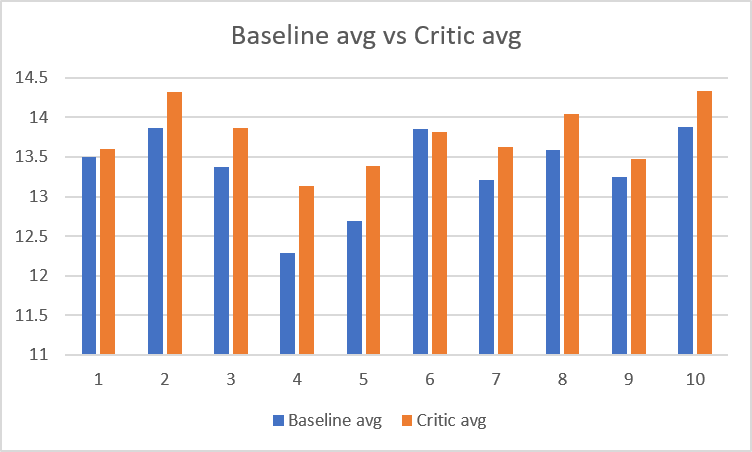
\includegraphics[width=0.8\linewidth]{../overall/Baseline-avg-vs-Critic-avg.png}
    \caption{Baseline vs CriticPilot Image Quality Average Score Comparison}
    \label{fig:AvgScore}
\end{figure}

\begin{figure}[htbp]
    \centering
    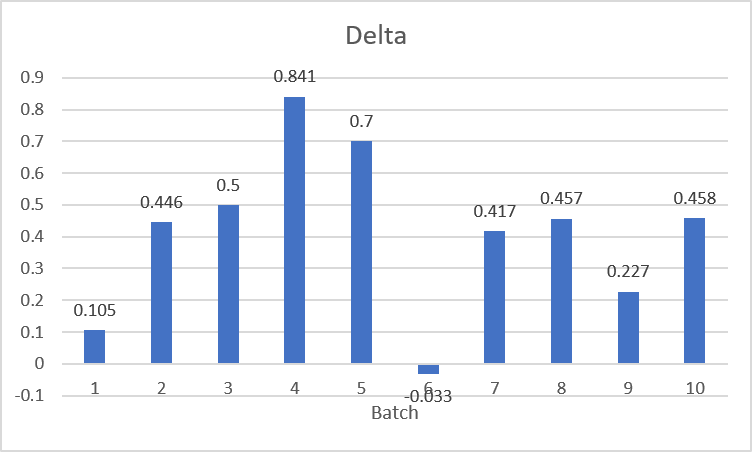
\includegraphics[width=0.8\linewidth]{../overall/Delta.png}
    \caption{CriticPilot Relative to Baseline Image Quality Average Score Difference}
    \label{fig:ScoreDelta}
\end{figure}

\subsection{Computational Overhead and
Efficiency}\label{computational-overhead-and-efficiency}

Typically, retry and reset mechanisms introduce additional computational
overhead. However, experimental data shows that
CriticPilot\textquotesingle s average evaluation rounds are 41.5, lower
than the baseline\textquotesingle s 43, an average reduction of
\textbf{1.5 rounds}. The reason is that L1 and L3 serve a dual role of
"pruning" and "navigation": local retry prevents invalid low-score
rounds from being counted and wasting subsequent optimization; global
reset decisively terminates stagnant paths, redirecting computational
resources to a broader search space.

\begin{figure}[htbp]
    \centering
    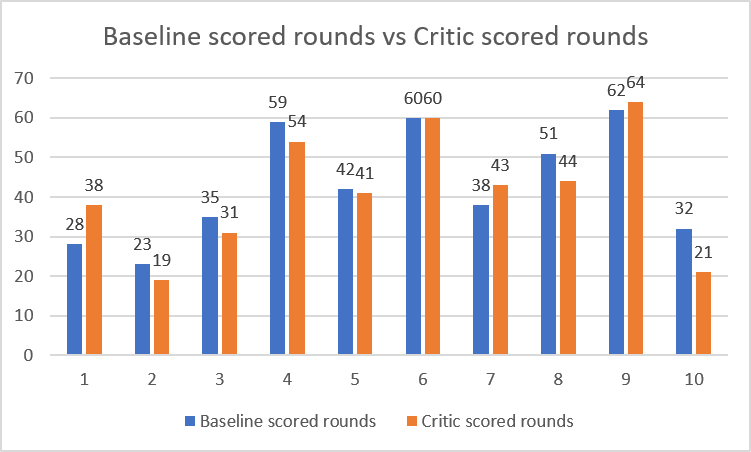
\includegraphics[width=0.8\linewidth]{../overall/Baseline-scored-rounds-vs-Critic-scored-rounds.png}
    \caption{Baseline vs CriticPilot Average Evaluation Rounds}
    \label{fig:AvgRounds}
\end{figure}

\begin{figure}[htbp]
    \centering
    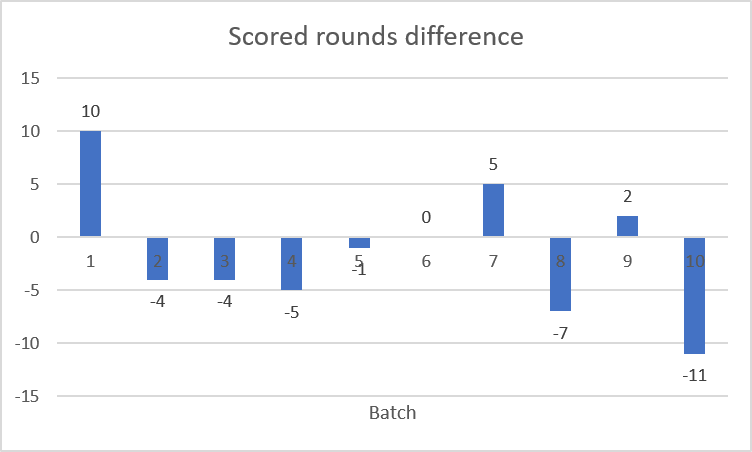
\includegraphics[width=0.8\linewidth]{../overall/Scored-rounds-difference.png}
    \caption{CriticPilot Relative to Baseline Average Evaluation Rounds Difference}
    \label{fig:RoundsDelta}
\end{figure}

\subsection{Mechanism Trigger
Frequency}\label{mechanism-trigger-frequency}

Statistics on average trigger counts per batch show: L1 triggers 14.2
times, L3 triggers 2.8 times. The high frequency of L1 triggers
indicates that low-quality candidates are frequently generated during
the original optimization process, and local retry provides an
inexpensive self-rescue mechanism. The lower but significant frequency
of L3 triggers---each global reset enables the system to break free from
erroneous history and gain opportunities to re-explore and find better
solutions (such as the significant score jump after L3 triggering in
Batch4). This frequency confirms that stagnation is not an occasional
phenomenon but an inherent drawback of linear optimization.

\begin{figure}[htbp]
    \centering
    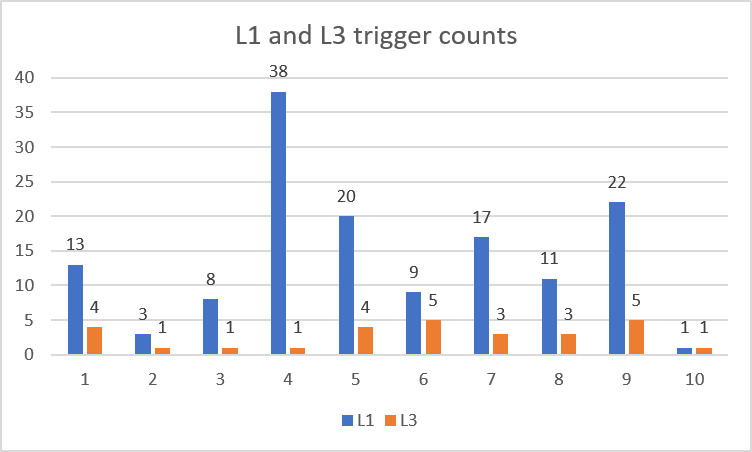
\includegraphics[width=0.8\linewidth]{../overall/L1-and-L3-trigger-counts.png}
    \caption{L1 and L3 Trigger Counts}
    \label{fig:TriggerCounts}
\end{figure}

\subsubsection{Case Analysis}\label{case-analysis}

\paragraph{Success Case A: Precise Counting Constraint
(Batch1)}\label{success-case-a-precise-counting-constraint-batch1}

\textbf{Original Prompt (excerpt)}: "A cabbage field with exactly 8
cabbages, each cabbage has dewdrops, and the field is covered with light
mist."

\textbf{Baseline Problem}: The number of cabbages generated frequently
deviates from 8, and dewdrops and mist are often lost, with scores
oscillating around 12.

\textbf{Mechanism Effect}: The error aggregator focuses errors on
"counting" and "visibility". Through repeated L1/L3 intervention, the
system evolves extremely strong hard constraints, for example: "\ldots{}
featuring exactly eight distinct cabbages, no more and no fewer. Every
cabbage must display visible dew droplets. A light veil of mist hangs
over the entire field \ldots". The highest score jumped from 13 to 15
(perfect score), successfully breaking the optimization ceiling.

\paragraph{Success Case B: Eliminating Object Hallucination
(Batch4)}\label{success-case-b-eliminating-object-hallucination-batch4}

\textbf{Original Prompt}: "A silver bracelet resting on a chessboard,
the bracelet is compact, not larger than one square."

\textbf{Baseline Problem}: Produced severe hallucinations, incorrectly
generating "stethoscopes" with tubular structures instead of "silver
bracelets", and the size was enormous, spanning multiple chessboard
squares.

\textbf{Mechanism Effect}: Error aggregation locked onto two core
issues: "incorrect object type" and "uncontrolled size". The system
generated highly targeted negative prompts (explicitly excluding
stethoscope components, such as "no chestpiece, no tubes") and utilized
spatial constraints with scene reference objects ("the bracelet must be
no larger than one chessboard square"). Hallucinations were stably
eliminated, significantly raising the lower bound of generation quality
and greatly reducing low-score rounds, thus Batch4\textquotesingle s $ \delta $
reached as high as +0.841.

\paragraph{Outlier Analysis: Batch6}\label{outlier-analysis-batch6}

Among all 10 batches, Batch6 is the only one with a negative $ \delta $ (-0.033).
Both achieved perfect scores of 15, and evaluation rounds were identical
(60 rounds), with differences only stemming from minor fluctuations in
candidate quality.

\textbf{Case Details}: The prompt required "A vintage fan with a rounded
base placed beside an antique knife on a wooden table". The baseline
performance was already strong, but Critic, to strengthen the
distinction between the fan and knife, adopted overly aggressive
exclusive descriptions (such as "loose circular fan head / no pedestal
base"), which deviated from the original prompt\textquotesingle s
inherent requirement for "rounded base", causing slight score decreases
in some rounds.

\textbf{Root Cause and Insights}: When the baseline already approaches
performance limits, or when the original prompt itself has semantic
ambiguity, Critic\textquotesingle s strong constraints may lead to
over-correction. This boundary condition reveals that future work could
introduce adaptive intervention strategies, appropriately reducing the
aggressiveness of retry and reset in later optimization stages to avoid
introducing new contradictions due to overfitting to error signals.
Overall, Batch6 should be regarded as "Critic essentially on par with
Baseline" rather than a significant failure.

\section{Conclusion}\label{conclusion}

This paper proposes CriticPilot, a lightweight extension to GenPilot
that addresses the problems of error overload and history pollution in
the linear optimization process by embedding a Planner-Critic mechanism.
Experiments validate the core value of CriticPilot:

\begin{enumerate}
\def\labelenumi{\arabic{enumi}.}
\item
  \textbf{Efficiency Without Cost}: Under the premise of reducing
  average evaluation rounds by 1.5, the average score improved by 0.4118
  points, proving that "quality control and error backtracking" is more
  important than "simply stacking iteration rounds".
\item
  \textbf{Dual Improvement of Upper and Lower Bounds}: L1 local retry
  suppresses low-score rounds, stabilizing the performance floor; L3
  global reset clears historical contamination, elevating the score
  ceiling.
\item
  \textbf{High Robustness}: Achieved positive gains in 90\% of test
  batches, with only one ambiguous scenario showing an acceptable minor
  regression, and no crashes occurred.
\end{enumerate}

In summary, CriticPilot, as a lightweight solution with minimal
architectural changes and no additional LLM calls, addresses the
problems of computational waste and stagnation in automated prompt
optimization with a high cost-effectiveness ratio. Future work will
explore adaptive intervention strategies to appropriately reduce the
aggressiveness of retry and reset in later optimization stages to avoid
introducing new contradictions due to over-correction.


\bibliography{iclr2026_conference}
\bibliographystyle{iclr2026_conference}

GenPilot Open Source Code: \url{https://github.com/27yw/GenPilot}

\appendix
\section{Appendix}

\subsection{Appendix A: Division of
Labor}\label{appendix-a-division-of-labor}

\begin{itemize}
\item
  \textbf{Li Zedong(李泽栋) 23307130271}: Designed experimental idea and
  plan, built basic project code framework ,wrote
  experimental report and made ppt
\item
  \textbf{Yan Haopeng(颜皓鹏) 24300240240}: Implemented CriticPilot
  code, executed testing, recorded data
\item
  \textbf{Shen Zixuan(沈子轩) 24300240213}: Analyzed data, organized
  results
\item
  \textbf{Zhu Yalun(朱雅伦) 24300240187}: Designed report
\end{itemize}

\end{document}
